%==============================================================================
%  Dhruv Kamdar - Analytics CV
%  Two-column template with circular photo (single page, A4)
%  Compile with: pdflatex Dhruv_Kamdar_CV.tex   (run twice)
%  Requires profile.png in the same folder.
%==============================================================================
\documentclass[a4paper,10pt]{article}

\usepackage[top=0cm,bottom=0cm,left=0cm,right=0cm]{geometry}
\usepackage[T1]{fontenc}
\usepackage[utf8]{inputenc}
\usepackage[scaled=0.92]{helvet}     % body sans (Nimbus Sans / Helvetica)
\usepackage{mathptmx}                % serif companion
\renewcommand{\familydefault}{\sfdefault}
\usepackage{xcolor}
\usepackage{tikz}
\usepackage{graphicx}
\usepackage{enumitem}
\usepackage{array}
\usepackage{fontawesome5}
\usepackage{eso-pic}
\usepackage[letterspace=150]{microtype}
\usepackage{hyperref}

\hypersetup{colorlinks=true,urlcolor=black,linkcolor=black,pdfborder={0 0 0},
            pdftitle={Dhruv Kamdar - CV},pdfauthor={Dhruv Kamdar}}

%------------------------------------------------------------------ palette --
\definecolor{bandcol} {HTML}{EFEDE9}   % header band + sidebar background
\definecolor{textcol} {HTML}{1B1B1B}
\definecolor{mutedcol}{HTML}{55534E}
\definecolor{rulecol} {HTML}{BDB9B2}
\definecolor{ringcol} {HTML}{CFC9C0}

\color{textcol}

%-------------------------------------------------------------- page metrics -
\newlength{\sidebarw}   \setlength{\sidebarw}{6.2cm}    % grey column width
\newlength{\bandh}      \setlength{\bandh}{4.55cm}      % header band height
\newlength{\sbtextw}    \setlength{\sbtextw}{4.35cm}    % sidebar text width
\newlength{\maintextw}  \setlength{\maintextw}{12.55cm} % main text width

%------------------------------------------------------------------- fonts ---
\newcommand{\namefont}[1]{{\fontfamily{ppl}\selectfont\fontsize{27}{29}\selectfont
  \textls[40]{#1}}}
\newcommand{\rolefont}[1]{{\fontsize{9}{11}\selectfont\color{mutedcol}
  \textls[300]{\MakeUppercase{#1}}}}
\newcommand{\datefont}[1]{{\fontsize{7.8}{9.5}\selectfont\itshape\color{mutedcol}#1}}

\newcommand{\heading}[2]{% #1 = rule width, #2 = title
  \par\vspace{6pt}\noindent
  {\fontsize{9.4}{11}\selectfont\bfseries\textls[190]{\MakeUppercase{#2}}}%
  \par\vspace{3pt}\noindent
  \textcolor{rulecol}{\rule{#1}{0.5pt}}\par\vspace{3pt}}

\newcommand{\sbhead}[1]{\heading{\sbtextw}{#1}}
\newcommand{\mnhead}[1]{\heading{\maintextw}{#1}}

%------------------------------------------------------------------ entries --
% \job{role}{organisation, location}{dates}
\newcommand{\job}[3]{%
  \par\noindent
  \begin{tabular*}{\maintextw}{@{}p{9.1cm}@{\extracolsep{\fill}}r@{}}
    {\fontsize{9.6}{11.5}\selectfont\bfseries #1} & \datefont{#3}
  \end{tabular*}%
  \par\vspace{1.5pt}\noindent
  {\fontsize{8.7}{10.5}\selectfont\itshape\color{mutedcol}#2}\par\vspace{2pt}}

% \sbentry{qualification}{institution}{dates}
\newcommand{\sbentry}[3]{%
  \par\noindent{\fontsize{8.6}{10.4}\selectfont\bfseries #1}%
  \par\vspace{0.5pt}\noindent{\fontsize{8.3}{10.2}\selectfont #2}%
  \par\vspace{0.5pt}\noindent\datefont{#3}\par}

\newcommand{\sbline}[1]{\par\vspace{1.5pt}\noindent{\fontsize{8.1}{10.4}\selectfont #1}\par}

\newcommand{\contactline}[2]{%
  \par\vspace{2.8pt}\noindent
  \makebox[0.52cm][l]{\textcolor{mutedcol}{\fontsize{8.5}{8.5}\selectfont #1}}%
  \parbox[t]{3.8cm}{\fontsize{8.2}{10}\selectfont\raggedright #2}\par}

\setlist[itemize]{leftmargin=1.0em,labelsep=0.45em,itemsep=1.4pt,topsep=1pt,
  parsep=0pt,partopsep=0pt,
  label=\textcolor{rulecol}{\raisebox{0.25ex}{\rule{2.6pt}{2.6pt}}}}

\newenvironment{cvbullets}
  {\fontsize{8.7}{10.4}\selectfont\begin{itemize}}
  {\end{itemize}\vspace{1pt}}

\newcommand{\skillblock}[1]{\par\noindent{\fontsize{8.2}{11.3}\selectfont #1}\par}

\setlength{\parindent}{0pt}
\setlength{\parskip}{0pt}
\pagestyle{empty}

% ---- background: grey sidebar + full-width header band ----------------------
\AddToShipoutPictureBG*{%
  \begin{tikzpicture}[remember picture,overlay]
    \fill[bandcol] (current page.north west)
          rectangle ([xshift=\sidebarw]current page.south west);
    \fill[bandcol] (current page.north west)
          rectangle ([yshift=-\bandh]current page.north east);
  \end{tikzpicture}}

%==============================================================================
\begin{document}

% ============================== HEADER =======================================
\vspace*{0.72cm}
\noindent\hspace*{1.52cm}%
\begin{minipage}[c]{3.16cm}
  \begin{tikzpicture}
    \clip (0,0) circle (1.58cm);
    \node at (0,0) {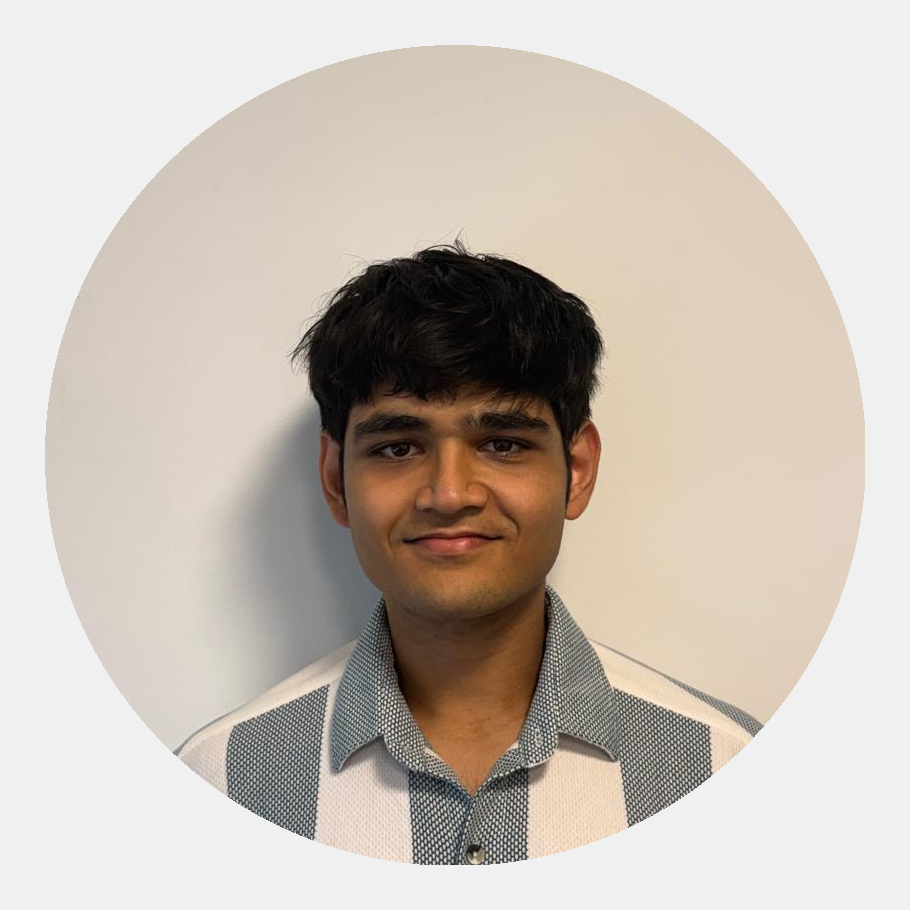
\includegraphics[width=3.6cm]{profile.png}};
    \draw[ringcol,line width=1.6pt] (0,0) circle (1.56cm);
  \end{tikzpicture}
\end{minipage}%
\hspace{2.22cm}%
\begin{minipage}[c]{12.7cm}
  \namefont{Dhruv Kamdar}\\[5pt]
  \rolefont{Data \& Business Analyst}\\[3pt]
  {\fontsize{8.2}{10}\selectfont\color{mutedcol}MSc Finance Analytics,
   King's College London \ \textbar\ \ Full UK Right to Work (Graduate Visa)}
\end{minipage}

\vspace{1.02cm}

% ============================== BODY =========================================
\noindent\hspace*{1cm}%
\begin{minipage}[t]{\sbtextw}
%------------------------------------------------------------------ SIDEBAR --
\vspace{0pt}

\sbhead{Contact}
\contactline{\faPhone*}{+44 7423 238207}
\contactline{\faEnvelope}{\href{mailto:kamdardhruv8@gmail.com}{kamdardhruv8@gmail.com}}
\contactline{\faMapMarker*}{London, United Kingdom}
\contactline{\faLinkedin}{\href{https://www.linkedin.com/in/dhruv-kamdar-254472363/}{linkedin.com/in/dhruv-kamdar}}
\contactline{\faGlobe}{\href{https://kamdardhruv8-droid.github.io/}{kamdardhruv8-droid.github.io}}

\sbhead{Education}
\sbentry{MSc Finance Analytics}{King's College London, UK}{Sep 2025 -- Sep 2026}
\sbline{\textbf{Modules:} Econometrics, Statistical Modelling, Data Analytics,
  Big Data \& Text Analytics, Financial Reporting}
\sbline{\textbf{Dissertation:} Built and backtested a systematic trading strategy
  in Python on large financial datasets}
\vspace{5pt}
\sbentry{BCom (GPA 8.7/10)}{Jai Hind College, Mumbai, India}{Mar 2022 -- Mar 2025}

\sbhead{Technical Skills}
\skillblock{Python -- Pandas, NumPy, Matplotlib\\
SQL -- querying, joins, validation\\
R -- data cleaning \& analysis\\
Excel -- PivotTables \& VLOOKUP\\
BI Dashboards \& Data Visualisation\\
Bloomberg Terminal\\
Git \textbar\ n8n \textbar\ LangGraph}

\sbhead{Analytics Toolkit}
\skillblock{Data Cleaning \& Validation\\
Exploratory Data Analysis\\
Statistical Modelling \& Inference\\
Experiment Design \& A/B Testing\\
Customer Segmentation\\
Reporting \& Process Automation\\
Stakeholder Communication}

\sbhead{Certifications}
\skillblock{\textbf{DeepLearning.AI}\\
\textit{Agentic AI Certificate}\\[3pt]
\textbf{Forage Simulations}\\
\textit{Goldman Sachs \textbar\ Quantium}}

\end{minipage}%
\hspace{1.55cm}%
\begin{minipage}[t]{\maintextw}
%--------------------------------------------------------------------- MAIN --
\vspace{0pt}

\mnhead{Professional Profile}
{\fontsize{8.8}{11.2}\selectfont
MSc Finance Analytics graduate who turns large, messy datasets into decisions senior
stakeholders act on. Strong across the full analytics cycle: cleaning and validation,
exploratory analysis, statistical modelling and dashboard reporting in Python, SQL, R and
Excel. Experienced leading teams and translating technical findings for non-technical
audiences. Available immediately for data and business analyst roles.\par}
\vspace{2pt}

\mnhead{Experience}

\job{Student Consultant --- Research Lead}{Practera Finance Micro Internship, London, UK}{Jun 2026 -- Jul 2026}
\begin{cvbullets}
\item Analysed \$77B+ of financial data from multiple sources to identify investment
      trends, uncovering a critical insight that redirected the team's entire
      recommendation approach.
\item Gathered, validated and reconciled data with an 8-person cross-functional team,
      ensuring quality and consistency across all deliverables.
\item Presented evidence-based recommendations directly to the client's Managing
      Director, translating complex analysis into clear, actionable insight.
\item Managed four concurrent workstreams to deadline, adapting the analytical approach
      mid-project when initial assumptions proved flawed.
\end{cvbullets}

\vspace{3pt}
\job{Intern --- Data \& Systems}{DG Software, Mumbai, India}{Mar 2025 -- Aug 2025}
\begin{cvbullets}
\item Improved data integrity by 30\% across 12 database tables by redesigning the data
      architecture and embedding automated validation processes.
\item Wrote SQL to query, extract, validate and reconcile datasets of 10,000+ records,
      improving retrieval efficiency by 25\%.
\item Built reporting dashboards and BI outputs used by senior management for operational
      decision-making, eliminating 8+ hours of weekly manual processing.
\end{cvbullets}

\mnhead{Analytics Projects}

\job{Team Leader --- King's Investment Fund}{Equity portfolio, UK \& European markets}{Mar 2026 -- Jun 2026}
\begin{cvbullets}
\item Led an 8-member team; delivered +300 to +500 bps outperformance versus the FTSE 100
      by applying CAPM and factor analysis to evaluate risk-adjusted returns.
\item Built performance dashboards in Python and Excel and presented strategy
      recommendations to faculty advisors.
\end{cvbullets}

\vspace{3pt}
\job{Quantium Data Analytics Simulation}{Forage --- retail sector}{Aug 2026}
\begin{cvbullets}
\item Cleaned and analysed 264,000+ retail transaction records in R and Python, delivering
      customer segmentation, brand affinity analysis and experiment design in a
      client-ready report for non-technical stakeholders.
\end{cvbullets}

\vspace{3pt}
\job{Agentic AI Workflow Automation}{Personal project}{Jun 2026 -- Present}
\begin{cvbullets}
\item Built automated data pipelines in Python, n8n and LangGraph for retrieval,
      validation and structured report generation, cutting manual research from hours
      to minutes.
\end{cvbullets}

\mnhead{Additional}
\begin{cvbullets}
\item \textbf{Goldman Sachs Operations Simulation (Forage), Aug 2026} --- analysed trade
      settlement data across Trading, Compliance and Technology teams.
\item \textbf{48-Hour Startup Challenge, King's College London, Nov 2025} --- gathered
      insight from 40+ users under deadline and pitched to a panel of senior mentors.
\end{cvbullets}

\end{minipage}

\end{document}
